\documentclass[12pt]{report}
\usepackage[T1]{fontenc}

\usepackage{anysize}
\marginsize{5em}{5em}{2em}{3em} % page margins, left, right, top, bottom
\usepackage{amsfonts, amsmath, amssymb, amsthm} % math stuff
\usepackage{graphicx} % images
\graphicspath{ {./graphics/} }

\author{CxRedix}

\newcommand{\bgap}{\vspace{4em}} % big gap
\newcommand{\sgap}{\vspace{2.2em}} % small gap
\newcommand{\tgap}{\vspace{1.5em}} % tiny gap


\begin{document}


\begin{center}
    \Large\textbf{CxRedix's Mathematics Cheatsheet}
\end{center}

This cheatsheet serves as a collection of mathematical constructs
that I found useful over the course of my learning.

Most of the stuff shown here does not try to explain a certain concept
in detail. It rather tries to \emph{supplement} you in remembering the most
\emph{important aspects} of the given mathematical construct within a certain
context.

\begin{center}
    
\includegraphics[width=25em, height=25em]{title_graphics}
\end{center}

\begin{center}
    \emph{Enjoy!}
\end{center}



\pagebreak
\chapter{Format of This Cheatsheet}

I personally believe having a consistent format would help aid readers
in obtaining information regarding a certain topic, and will also help the author(me)
in writing concepts without missing certain details within a concept:

\vspace{3em}

Each new introduction of a \textbf{new concept} will have the following:
\begin{enumerate}
    \item A hopefully \textbf{detailed overview} of the concept in general.
    \item The \textbf{technical definition / mathematical term} of such a concept.
    \item \textbf{Example use-cases and explanation} of the use-case of such a concept.
\end{enumerate}

\tgap

\emph{And \textbf{optionally}}:
\begin{enumerate}
    \item Some relevant / interesting \textbf{notes} regarding the concept.
    \item Additional resources as \textbf{footnotes} to explain the concept in more detail.
    \item If the mathematical definition has fancy letters and symbols, it will get explained
        in the "\textbf{where}" section right after the definition.
    \item \textbf{Counter-examples and explaination} of why it doesn't work this way.
        (It's optional because sometimes counter-examples are harder to explain)
\end{enumerate}

\tgap

\emph{For \textbf{text formatting}}:
\begin{enumerate}
    \item Important / Relevant new words for concepts will get their fonts \textbf{bolded}.
\end{enumerate}





\newpage
\tableofcontents

\newpage
\chapter{Operation Properties}

\section{Associative Property}
Statement:
A binary operation $*$ on set $S$ is associative iff changing the order of which the operations are performed
does not change the result.

\begin{center}
    $(x * y) * z = x * (y * z), \forall x,y,z \in S$
\end{center}



\section{Commutative Property}
Statement:
A binary operation $*$ on set $S$ is commutative iff changing the order of the operands does not change
the result.

\begin{center}
    $x * y = y * x, \forall x,y \in S$
\end{center}

\section{Anti-Commutative Property}
Statement:
A binary operation $*$ on set $S$ is anti-commutative iff changing the order of the operands negates the original
result.

\begin{center}
    $x * y = -(y * x), \forall x,y \in S$
\end{center}



\newpage
\chapter{Range Manipulation}

\section{Intervals}
TODO: explain mathematical definitions of intervals [a, b], (a, b) and in between
explain how to do operations on them, and what they meant intuitively...

Explain how intervals can be applied in functions to give a more complicated inter al

Explain the limitations of intervals in terms of mathematical expression; Intervals can't explain distribution of values within it.
It only explains the bounds.

\section{Useful Manipulations}
\subsection{Linear Mapping}
Given some value $x \in [a, b]$, we wish to map all values linearly to another range such that $x' \in [i, j]$,
we can follow this procedure(assuming that $a, b, i, j \in \mathbb{R}$):

\begin{enumerate}
    \item Shift $x$ from $[a, b]$ to $[0, (b - a)]$ by subtracting by $a$.
    \item Squeeze the value to range $[0, 1]$ by dividing by $(b - a)$.
    \item Scale the range $[0, 1]$ to $[0, (j - i)]$ by multiplying by $(j - i)$.
    \item Finally, offset the range $[0, (j - i)]$ to the desired range $[i, j]$ by adding $i$.
\end{enumerate}

In mathematical terms:
\begin{center}
    $m(x, a, b, i, j) = \frac{(x - a)(j - i)}{(b - a)} + i$
\end{center}

Very useful for mapping a value from one range to another!

This also works for ranges that are reversed(i.e. not following the $[min, max]$ format)! So for instance, let's map
from $[20, 30]$ to $[1, 0]$:
\begin{center}
    \begin{flalign}
        m(x, 20, 30, 1, 0) & = \frac{(x - 20)(0 - 1)}{(30 - 20)} + 1 \\
                           & = \frac{20 - x}{10} + 1 \\
                           & = \frac{20 - x + 10}{10} \\
                           & = \frac{30 - x}{10}
    \end{flalign}
\end{center}

We can check for it's validness by putting this in a graphing calculator like \textbf{Desmos}:
\begin{center}
    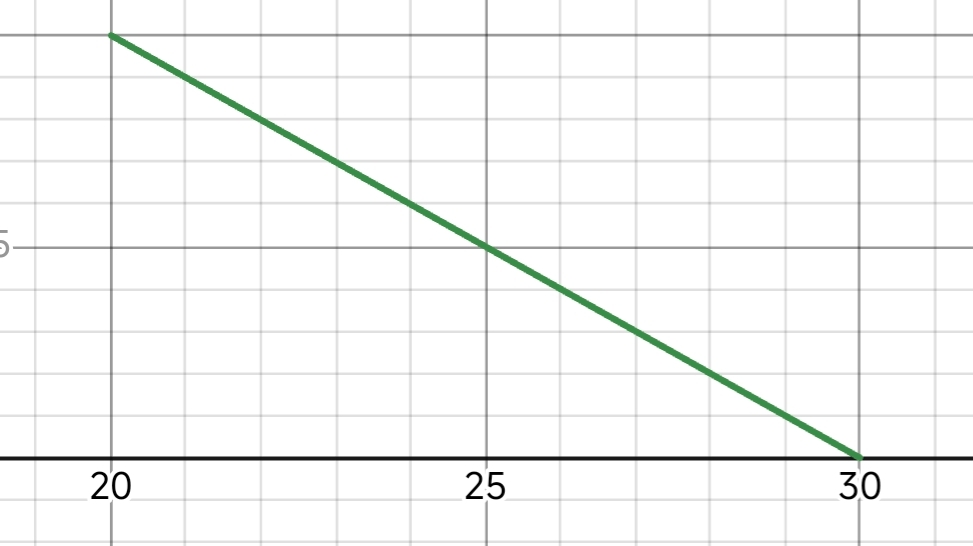
\includegraphics[width=25em, height=13em]{linear_mapping_reversed_example}
\end{center}

You can see $20$ points to $1$, and $30$ points to $0$ with a smooth linear line in between!

In fact, linear mapping formula used here is actually solving for a line formula,
where two points are $(20, 1)$ and $(30, 0)$ :D



\sgap
Here are some pre-derived formulas for common range mappings:

\tgap
From $x \in [a, b]$ to $x' \in [0, 1]$ (Also called the normal range)
\begin{center}
    $x' = \frac{x - a}{b - a}$
\end{center}

\sgap
From $x \in [a, b]$ to $x' \in [-1, 1]$ (Also called the signed normal range)
\begin{center}
    $x' = \frac{2(x - a)}{b - a} - 1$
\end{center}

\subsection{Value Clamping}
Sometimes we want to restrict some value $x \in \mathbb{R}$ within some max or a min boundary, we can utilize exactly
the $\max$ and $\min$ functions for this exact purpose! They are defined as follows:

\sgap
\begin{samepage}
    Here is the definition of the $\max$ function:
    \begin{center}
        \[
            \max(x, y) =
            \begin{cases}
                x & \text{if } x \geq y \\
                y & \text{if } x < y
            \end{cases}
        \]
    \end{center}
\end{samepage}

It gives you the max between two numbers $x, y \in \mathbb{R}$, pretty straight forward!

We can restrict values to not get below a certain value by utilizing this function, for instance
$\max(x, 20)$ forces the result to be greater of equal to $20$, in other words $\max(x, 20) \geq 20$. If $x$
goes below $20$, the $\max$ function always just picks $20$, otherwise it picks $x$ since it's greater.

\sgap

\begin{samepage}
    And this is the definition of $\min$ function:
    \begin{center}
        \[
            \min(x, y) =
            \begin{cases}
                x & \text{if } x \leq y \\
                y & \text{if } x > y
            \end{cases}
        \]
    \end{center}
\end{samepage}

Similar to $\max$ but reversed. It gives the minimum of two values $x, y \in \mathbb{R}$.

We can restrict values to not get above a certain value, for example:
$\min(x, 100)$, the result will never get above $100$, since if $x$ is greater than $100$, that would mean
$\min$ will just pick $100$ since it's smaller. Otherwise it'll pick $x$.


\sgap
Finally, we can utilize both to restrict a value $x \in \mathbb{R}$ within a certain range $[a, b]$ by using both one after the other.
This is often called \textbf{clamping}:
\begin{center}
    $clamp(x, a, b) = \min(\max(x, a), b)$
\end{center}

We first restrict $x$ to not get below $a$, then we restrict that result to not get above $b$ :D


\subsection{Value Stepping}
TODO


\subsection{Looping a Range}
If you have a value $x \in \mathbb{R}$, and you wish to do something to it, so it always stay in a range of $[a, b]$,
then you can follow the following procedure:

TODO







\newpage
\chapter{Bounds, Minimum and Maximum}

\section{Finding Tight Intervals}
Recall the definition of $\min$ and $\max$ functions from the chapter \textbf{Range Manipulation}'s \textbf{Value Clamping} section.

We can generalize the $\min$ and $\max$ function to include more values :3

For $\min$:
\begin{center}
        $\min(a_1, a_2, a_3, ..., a_n) = \min(a_1, \min(a_2, a_3, ..., a_n))$
\end{center}

And for $\max$:
\begin{center}
        $\max(a_1, a_2, a_3, ..., a_n) = \max(a_1, \max(a_2, a_3, ..., a_n))$
\end{center}

For example, $\min(1, 4, -4) = \min(1, \min(4, -4))$. Here we can evaluate from the inside to the outside.
So $\min(4, -4) = -4$ and finally $\min(1, -4) = -4 = \min(1, 4, -4)$. Same should apply to the generalized $\max$ function!

In other words:
\begin{itemize}
    \item $\min$: Returns the minimum among all the values $a_i$.
    \item $\max$: Returns the maximum among all the values $a_i$.
\end{itemize}

By using this generalized $\min$ and $\max$ functions, we can actually find the bounding range of a set of values,
for example, if we have a set of values denoted by $a_i$, and there are $n$ of them (i.e. the first element is $a_1$ and last is $a_n$),
then, the interval that \textbf{tightly} includes all values is defined as:
\begin{center}
    $[\min(a_1, a_2, a_3, ..., a_n), \max(a_1, a_2, a_3, ..., a_n)]$
\end{center}

For example, if we have values $1, 4, 5, -2, 3$, we can find it's tight bound as:
\begin{center}
    $[\min(1, 4, 5, -2, 3), \max(1, 4, 5, -2, 3)] = [-2, 5]$
\end{center}

Here's how it looks like when plotted in the real number line:

TODO: an image here demonstrating the example :3



\section{Finding Bounds in Higher Dimensions}
This can be very useful if we extend this to two or more dimensions, for instance, we can find the bounding box in two dimensions
given a bunch of points by finding the $\min$ and $\max$ of all points:

TODO: axis-aligned bounding boxes etc.







\newpage
\chapter{Trigonometry}
As the name suggests, "tri"-gonometry is the study of triangles :3, why triangles?
Because triangles is the most "simplest" geometry that you can construct with line segments!

Triangles can also be used to "approximate" / "re-construct" into other shapes, so it is very
important to study all the properties regarding triangles.

TODO:
fill in regular cos, sin, tan, cot, sec. Also fill in identities and properties.




\newpage
\chapter{Handedness and Chirality}

TODO




\newpage
\chapter{Linear Algebra}
Linear Algebra is the study of adding things together, it mainly studies two important concepts:

\begin{enumerate}
    \item it studies how the "same type" of things when added, results in
        a new thing that is of the "same type".

    \item It also studies if you can multiply a "number" to a type of
        thing, to produce a new thing of the same type.
\end{enumerate}

These "things" are then applicable by Linear Algebra, pretty cool concept!


\begin{center}
    
\includegraphics[width=13em, height=13em]{linear_algebra_core}
\end{center}

\section{Vectors}

\subsection{Vector Spaces}

In an abstract sense, a \textbf{vector} is any element inside a valid \textbf{vector space}. So what is a vector space? It is simply a group of things that satisfies the following properties:

If we have vectors in vector space $S$, then those vectors should
satisfy the following axioms of addition and scalar multiplication:

\sgap
\paragraph{For Addition:}
\begin{enumerate}
    \item Closed under addition: For all $\vec{x}, \vec{y} \in S$ such that $\vec{x} + \vec{y} \in S$.
    \item Commutative law: For all $\vec{x}, \vec{y} \in S$ such that $\vec{x} + \vec{y} = \vec{y} + \vec{x}$.
    \item Associative law: For all $\vec{x}, \vec{y}, \vec{z} \in S$ such that $(\vec{x} + \vec{y}) + \vec{z} = \vec{x} + (\vec{y} + \vec{z})$.

    \item Existence of an additive identity: $\exists \vec{0} \in S, \forall \vec{v} \in S (\vec{v} + \vec{0} = \vec{v})$.
    \item Existence of an additive inverse: $\forall \vec{v} \in S (\vec{v} + (-\vec{v}) = \vec{0})$ where $\vec{0}$ is the additive identity.
\end{enumerate}

\sgap
\paragraph{For Scalar Multiplication, If $a,b \in \mathbb{R}$ and $\vec{x}, \vec{y}, \vec{z}$ is in vector space $S$ then:}
\begin{enumerate}
    \item Closed under scalar multiplication: $a\vec{v} \in S$
    \item Distributive law for scalar: $a(\vec{x} + \vec{y}) = a\vec{x} + a\vec{y}$
    \item Distributive law for vector: $(a + b)\vec{x} = a\vec{x} + b\vec{x}$

    \item Scalar Associative law: $a(b\vec{x}) = (ab)\vec{x}$
    \item Scalar multiplicative identity with 1: $1\vec{x} = \vec{x}$
\end{enumerate}\footnote{Make the syntax of this to be consistent with everything above}

That is a lot of rules to satisfy!
Anyhow, the most important space is $\mathbb{R}^n$, but at least know
that all of linear algebra, can be also applied to other
vector spaces(such as functions, or polynomials) as well!


\subsection{Geometric Representation of Vectors}
it's geometric representation states that a \textbf{vector} is a \textbf{directed segment} that can be used to indicate \textbf{relative displacement}:

\begin{center}
    
\includegraphics[width=13em, height=13em]{geometric_vector_desc}
\end{center}


\begin{itemize}
    \item $tail$: the start of the vector; can be understood as where this vector is coming from.
    \item $head$: the end of the vector; can be understood as where this vector displaces to.
    \item $magnitude$ / $length$: It's magnitude / length represents the amount of displacement, it's always non-negative,
        that is $\forall \vec{v} (\|\vec{v}\| \geq 0)$
    \item $direction$: A vector has a direction it's pointing towards.
\end{itemize}

\vspace{.5em}

\emph{
    NOTE: a vector does not have a position, it's always relative to something.
    In other words, you can move the vector tail along with it's head everywhere as you see fit.
}


\subsection{The Very Important $\mathbb{R}^n$ Vector Space}
A $\mathbb{R}^n$ vector denotes a list of real numbers $\mathbb{R}$, it's mathematical definition is as follows:

\paragraph{as a row vector:}
\begin{center}
    $\vec{v}=[a_1~a_2~a_3~...~a_n]$
\end{center}

\paragraph{or as a column vector:}
\begin{center}
    \[
        {\vec{v}} = \begin{bmatrix}a_1 \\ a_2 \\ a_3 \\ \vdots \\ a_n\end{bmatrix}
    \]
\end{center}

where:
\begin{itemize}
    \item $\vec{v}$: is the vector itself.
    \item $n$: denoting the \textbf{dimensions} of the vector.
    \item $a_i$: denoting the \textbf{$i$th} term of the vector.
    \item $\mathbb{R}^n$: denoting the "vector space"
\end{itemize}

\vspace{.5em}

\emph{
    NOTE: $i$ is often called the "index" or "subscript" of an element. For instance:
    "$a_1$", here $1$ is the index that refers to the first element (assuming you start with $1$)
}

\sgap


\subsection{$\mathbb{R}^n$ Vector Properties}

\textbf{Magnitude} of a vector in Eucledian Space(also referred to as Eucledian / Pythagorean Distance):
\begin{center}
    \[
        \|\vec{v}\|=\|\begin{bmatrix}a_1 \\ a_2 \\ a_3 \\ \vdots \\ a_n\end{bmatrix}\|=\sqrt{a_1^2+a_2^2+a_3^2+...+a_n^2}
    \]
\end{center}

As the name "Pythagorean Distance" suggests, the magnitude of a vector can be seen as the hypotenuse of a right triangle if we
decompose it's axis individually. In which we can apply the pythagorean therorem to get the eucledian distance / length of the hypotenuse.

\sgap
\begin{samepage}
    A vector is said to be a \textbf{zero vector} if it's magnitude is exactly $0$:
    \begin{center}
        \[
            \|\vec{v}\|=0 \iff \vec{v}=\vec{0}=\begin{bmatrix}0 \\ 0 \\ \vdots \\ 0\end{bmatrix}
        \]
    \end{center}

    The zero vector can be used to denote "no displacement" and it is an \textbf{additive identity}, in mathematical terms:
    \begin{center}
        \[
            \exists \vec{k} \forall \vec{v}(\vec{k}+\vec{v}=\vec{v})
        \]
    \end{center}

    Here's $\vec{k}$ represents additive identity, which is exactly the zero vector $\vec{0}$.
\end{samepage}


\sgap

\begin{samepage}
        A vector is said to be a \textbf{unit vector} if it's magnitude is exactly $1$:
        \begin{center}
            \[
                \|\vec{v}\|=1
            \]
        \end{center}

        Which we can denote this unit vector as a letter with a "hat" ("$\hat{v}$") indicating that it is a unit vector.

        Any non-zero vector($\|\vec{v}\| \neq 0$) can be turned into a unit vector by utilizing \textbf{Scalar Division}. (see section \textbf{Vector Operations} for more detail)

        A unit vector is very special as it can both mean "pure direction" or "a direction with a controllable magnitude".
\end{samepage}

\sgap



\subsection{$\mathbb{R}^n$ Vector Operations}

\textbf{Addition} and \textbf{Subtraction} of two vectors:
\begin{center}
    \[
        {\vec{a}}\pm{\vec{b}}=\begin{bmatrix}a_1 \\ a_2 \\ \vdots \\ a_n\end{bmatrix} \pm \begin{bmatrix}b_1 \\ b_2 \\ \vdots \\ b_n\end{bmatrix}=\begin{bmatrix}a_1 \pm b_1 \\ a_2 \pm b_2 \\ \vdots \\ a_n \pm b_n\end{bmatrix}
    \]
\end{center}

\vspace{.5em}

\emph{
    NOTE: The add and subtract operations of vectors are also known as "element-wise" operations.
Because they do each operation for each element with the same index from both vectors.
(Same principle should apply for both column and row vectors)
}

\sgap

\textbf{Scalar Multiplication} of a vector and a scalar:
\begin{center}
    \[
        {\vec{a}}k=k{\vec{a}}=k \begin{bmatrix}a_1 \\ a_2 \\ \vdots \\ a_n\end{bmatrix}=\begin{bmatrix}ka_1 \\ ka_2 \\ \vdots \\ ka_n\end{bmatrix}
    \]
\end{center}

Scaling a vector by a scalar $k$ applies that scalar for every single element, which in turn scales the vector's magnitude by exactly $k$, in mathematical terms:
\begin{center}
    $\|k\vec{a}\|=k\|\vec{a}\|$
\end{center}

This can be utilized to scale a unit vector $\hat{n}$ by a desired amount of magnitude, since a unit vector's magnitude is defined as $1$, in mathematical terms:
\begin{center}
    $\|k\hat{n}\| = k$
\end{center}

Scaling a unit vector by a scalar $k$ simply just makes it have exactly the magnitude of $k$.


\sgap

\textbf{Scalar Division} of a vector and a scalar:
\begin{center}
    \[
        \vec{a}=\begin{bmatrix}a_1 \\ a_2 \\ \vdots \\ a_n\end{bmatrix},\frac{\vec{a}}{k}=\begin{bmatrix}\frac{a_1}{k} \\ \frac{a_2}{k} \\ \vdots \\ \frac{a_n}{k}\end{bmatrix}
    \]
\end{center}

This can be utilized to turn any non-zero vector into it's unit vector version by dividing the vector with it's own magnitude:
\begin{center}
    \[
        {\hat{a}}=\frac{\vec{a}}{\|\vec{a}\|}
    \]
\end{center}

\vspace{.5em}

\emph{
    NOTE: both \textbf{Scalar Multiplication} and \textbf{Scalar Division} are "inverse" of each other, in mathematical terms:
}
\begin{center}
    \[
        \frac{k\vec{v}}{k}=\vec{v}
    \]
\end{center}

Applying the same scalar multiplied and divided gives back the original vector.



\sgap

\textbf{Inner Product / Dot Product}(also known as projection product) of two vectors:
\begin{center}
    \[
        {\vec{a}} \cdot {\vec{b}}=\langle \vec{a}, \vec{b} \rangle=\begin{bmatrix}a_1 \\ a_2 \\ \vdots \\ a_n\end{bmatrix} \cdot \begin{bmatrix}b_1 \\ b_2 \\ \vdots \\ b_n\end{bmatrix}=a_1b_1+a_2b_2+a_3b_3+...+a_nb_n
    \]
\end{center}

If we have an angle $\theta$ between two vectors, the inner / dot product of two vectors can be rewritten as
\begin{center}
    \[
        {\vec{a}} \cdot {\vec{b}}=\langle \vec{a}, \vec{b} \rangle=\|\vec{a}\|\|\vec{b}\|cos~\theta
    \]
\end{center}

The dot / inner product of two vectors $\vec{a}$ and $\vec{b}$ can be seen as the \textbf{length of the projection} of either $\vec{a}$ to $\vec{b}$ or vice versa(since dot product is commutative).

If $\vec{a}$ and $\vec{b}$ are both unit vectors (i.e. $\|\vec{a}\| = 1, \|\vec{b}\| = 1$), then the above equation
can be simplifed to $\hat{a} \cdot \hat{b}=cos~\theta$.

\vspace{.5em}

\emph{
    NOTE: the dot / inner product is actually not a multiplication between two vectors due to the fact that
    it returns a \textbf{scalar}, and not a \textbf{vector}. If one has to define multiplication, it has to satisfy the following:
    $\vec{x} * \vec{y} = \vec{z} ~~ x,y,z \in \mathbb{S}^n$
    but dot / inner product does this:
    $\vec{x} * \vec{y} = s ~~ x,y \in \mathbb{S}^n, s \in \mathbb{R}$
    In laymans' terms, two apples multiplied togethers should give an apple, and not something else.
}

\sgap
\textbf{Cross Product}(also known as Vector Product / Directed Area Product) of two three-dimensional vectors in Eucledian space:
\begin{center}
    \[
        {\vec{a}} \times {\vec{b}}=\begin{bmatrix}x \\ y \\ z\end{bmatrix} \times \begin{bmatrix}i \\ j \\ k\end{bmatrix}=\begin{bmatrix}ky - jz \\ iz - kx \\ jx - iy\end{bmatrix}
    \]
\end{center}

The cross product of $\vec{a}$ to $\vec{b}$ returns a new vector $\vec{c}$ that is perpendicular to both vectors $\vec{a}$ and $\vec{b}$, it is
then a valid kind of multiplication for vectors :D

\sgap
\begin{samepage}
    Notice that, if you swap the operands, the result is entirely different:
    \begin{center}
        \[
            {\vec{b}} \times {\vec{a}}=\begin{bmatrix}i \\ j \\ k\end{bmatrix} \times \begin{bmatrix}x \\ y \\ z\end{bmatrix}=\begin{bmatrix}jz - ky \\ kx - iz \\ iy - jx\end{bmatrix}
        \]
    \end{center}
\end{samepage}

\begin{samepage}
    Therefore, it is actually \textbf{non-commutative} and actually is \textbf{anticommutative}:
    \begin{center}
        \[
            {\vec{a}} \times {\vec{b}} \neq {\vec{b}} \times {\vec{a}},~{\vec{a}} \times {\vec{b}}=-(\vec{b} \times \vec{a})
        \]
    \end{center}

    Due to this non-commutativeness, it's actually very strictly related to \textbf{chirality} / \textbf{handedness} of the given 3D / 7D space!
\end{samepage}

\begin{samepage}
    The following image regarding cross products uses a \textbf{Right-hand Coordinate System}:
    \begin{center}
        
\includegraphics[width=13em, height=13em]{vector_cross_product_righthanded}
    \end{center}
\end{samepage}


\sgap
\begin{samepage}
    If we define an angle $\theta$ between vectors $\vec{a}$ and $\vec{b}$, we can then find the magnitude of the cross product to be:
    \begin{center}
        \[
            {\|\vec{a}} \times {\vec{b}\|}=\|\vec{a}\|\|\vec{b}\| \lvert sin~\theta \rvert 
        \]
    \end{center}

    Notice that $sin~\theta$ is actually wrapped in absolute value, since the magnitude of a vector
    must always be non negative.

    The magnitude of the cross product is also equivalent to the area of the parallelogram formed by letting $\vec{a}$ and $\vec{b}$ be the two sides.

    \footnote{
        Cross product only exists in dimensions of 3 and 7 in Eucledian space, see this for more detailed formulation and proof:
        Cross Products of Vectors in Higher Dimensional Euclidean Spaces by W. S. Massey;
        The American Mathematical Monthly, Vol. 90, No. 10 (Dec., 1983), pp. 697-701.
    }
\end{samepage}

\subsection{Dot Product and Projections in $\mathbb{R}^n$}
TODO: explain how dot product does essentially projections of one vector $A$ ontop of the other vector $B$.



\subsection{$\mathbb{R}^n$ Vectors and Points in Eucledian Space}
In eucledian space, a point is defined as a tuple of values that define a unique position in space:\footnote{TODO: maybe move the definition of the point somewhere else?}
\begin{center}
    $P=\begin{pmatrix}p_1 & p_2 & p_3 & ... & p_n\end{pmatrix}$
\end{center}

A Vector on the other hand, represents a relative displacement, the point $P$ can actually be understood as the tip / head of the vector
after the \textbf{relative displacement} is applied from the \textbf{origin} of where $P$ resides in:
\begin{center}
    $\vec{P}=\begin{bmatrix}p_1 \\ p_2 \\ p_3 \\ ... \\ p_n\end{bmatrix}$
\end{center}

Notice that the elements $p_i$ are of equivalent values. Because a point is essentially the origin point
that got offset by some unique displacement(which can be represented by a vector).


\subsection{$\mathbb{R^n}$ Vector Decomposition}
TODO: decomposition to it's indivdual basis vectors...
Also explain uniqueness of decomposition


\subsection{$\mathbb{R}^n$ Basis Vectors}
Basis vectors refer to special vectors that denote a specific
TODO


\section{Homogeneous Coordinates}
TODO

\section{Matrix}
TODO

\subsection{Matrix Properties}
TODO

\subsection{Matrix Operations}
TODO

\subsection{Matrix as a Combination of Vectors}
TODO

\subsection{Matrix as a Representation of Systems of Linear Equations}
TODO

\subsection{Matrix as a Means of Linear Transformation}
TODO: explain Rotation, Scale, Shearing...

\subsection{Why is Translation not a form of Linear Transformation}
TODO: explain why translation is actually Shearing from a higher dimension projected down
to a dimension lower as translation...

\subsection{Matrix for Transforming Between Two Eucledian Spaces}
TODO

\subsection{Projection Matricies}
TODO

\subsection{Useful Matrix Constructs}
You can rotate an arbitrary point $A$ around another point $O$ by following these steps:
\begin{enumerate}
    \item Translate $O$ back to the origin, and bring $A$ with it.
    \item Rotate this new $A$ around the origin(which is also where the new $O$ resides)
        as how you would normally.
    \item Translate the new $O$ back to where $O$ originally was, and bring the new rotated $A$ with it.
    \item You now have your rotated $A$ around $O$!
\end{enumerate}

This can be further written in matrix if we promote $O$ and $A$ to homogeneous coordinates(to allow for translation),
in which the matrix $\textbf{T}$ represents translating $O$ back to origin, and matrix $\textbf{R}$ represents
some pure rotational matrix around the origin. Which can be written mathematically as:
\begin{center}
    $\textbf{M}=\textbf{T}^{-1}\textbf{R}\textbf{T}$
\end{center}

In which you can now apply the final matrix $\textbf{M}$ on any point $A$ which effectively rotates it around $O$!

\sgap
You can create a matrix to convert from one Eucledian space $A$ to Eucledian space $B$ by filling a matrix with
basis vectors per column of space $A$ relative to $B$, in mathematical terms:

TODO





\section{Primitive Geometry}
\subsection{Point}
In all of geometry, a point is the most basic geometrical primitive, it denotes a location relative to some space, it has no size
nor does it have any direction.

A point can be defined in eucledian space using the "\textbf{cartesian}" way of representing, which is commonly known as
\textbf{cartesian coordiantes}:
\begin{center}
    $P = \begin{pmatrix}a_1 & a_2 & a_3 & ... & a_n\end{pmatrix}$
\end{center}

where:
\begin{itemize}
    \item $P$: is the point itself :)
    \item $a_i$: is the magnitude of each basis vectors of this eucledian space.
    \item $n$: denotes the point residing in an $n$-th dimension eucledian space.
\end{itemize}

For example, in 3D cartesian coordinates, the point $\begin{pmatrix}1 & 2 & 3\end{pmatrix}$ 
(assuming we use $\hat{x}$, $\hat{y}$ and $\hat{z}$ as the basis vectors) would represent this:
\begin{enumerate}
    \item Begin in the origin of the 3D eucledian space: $\begin{pmatrix}0 & 0 & 0\end{pmatrix}$.
    \item Move $1$ unit in the $\hat{x}$ direction.
    \item Move $2$ units in the $\hat{y}$ direction.
    \item Move $3$ units in the $\hat{z}$ direction.
\end{enumerate}


\subsection{Line}
TODO

\subsection{Ray}
\begin{center}
    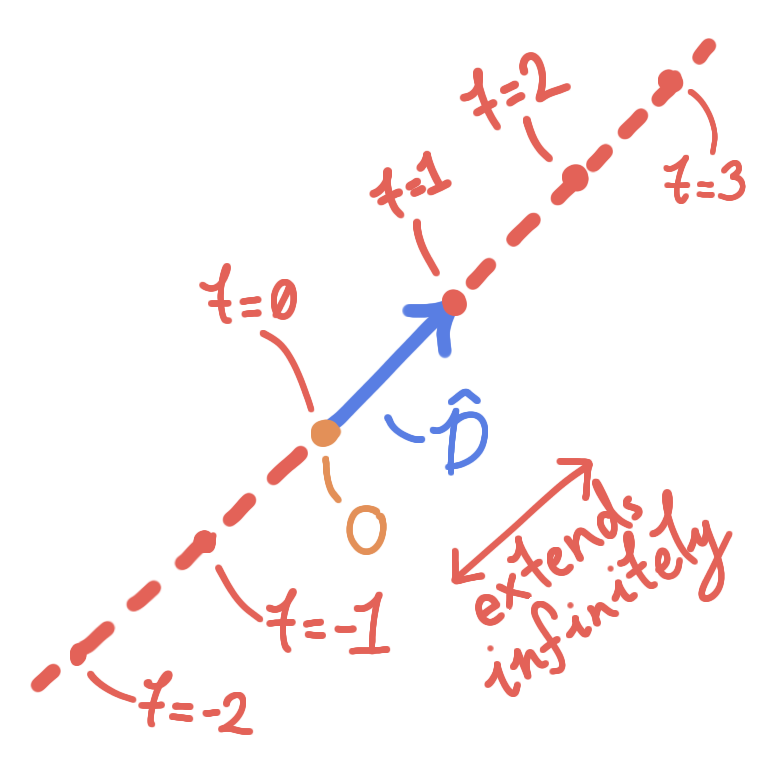
\includegraphics[width=13em, height=13em]{primitive_geometry_ray}
\end{center}

A \emph{ray} is defined as a directed segment that has a
\emph{origin}(a.k.a. having a position), and a \emph{direction}. It is mathematically defined as follows:

\begin{center}
    $P=O+\hat{D}t$
\end{center}

where:
\begin{itemize}
    \item $P$: is any point along the ray.
    \item $O$: is the origin of the ray, where it starts.
    \item $\hat{D}$: is the unit vector representing the direction of the ray.
    \item $t$: represents the percent / factor that "moves" the point along the ray.
\end{itemize}

If $t > 0$ then $P$ would be along the ray's direction $\hat{D}$.
If $t < 0$ then $P$ would be along the negative ray's direction $-\hat{D}$.
If $t = 0$ then $P$ would be exactly at the origin point $O$.

\subsection{Plane}
A plane can be defined in numerous ways.

\textbf{Distance-Normal form}:
\begin{center}
    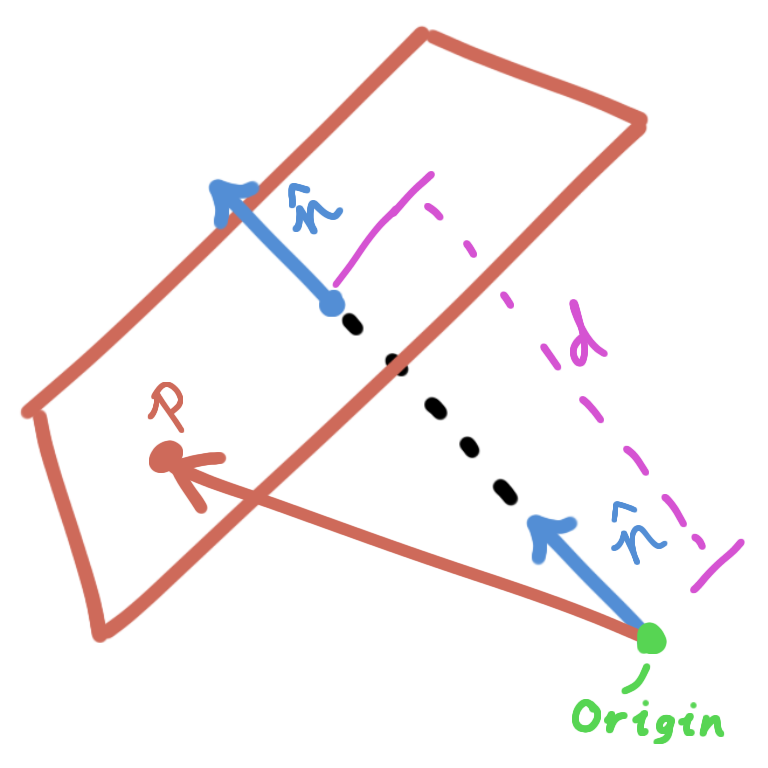
\includegraphics[width=13em, height=13em]{primitive_geometry_distance_normal_plane}
\end{center}

\begin{center}
    $P \cdot \hat{n} - d = 0$
\end{center}

where:
\begin{itemize}
    \item $P$: is any point on the plane.
    \item $\hat{n}$: is the unit vector that represents the direction / facing of the plane.
    \item $d$: is the offset / distance of the plane from the origin along the direction $\hat{n}$ where it is facing.
\end{itemize}

The plane is defined here as all the points that resides at an equal level of length
given a unit vector pointing in the direction in which it's facing.

\sgap

\textbf{Point-Normal form}:
\begin{center}
    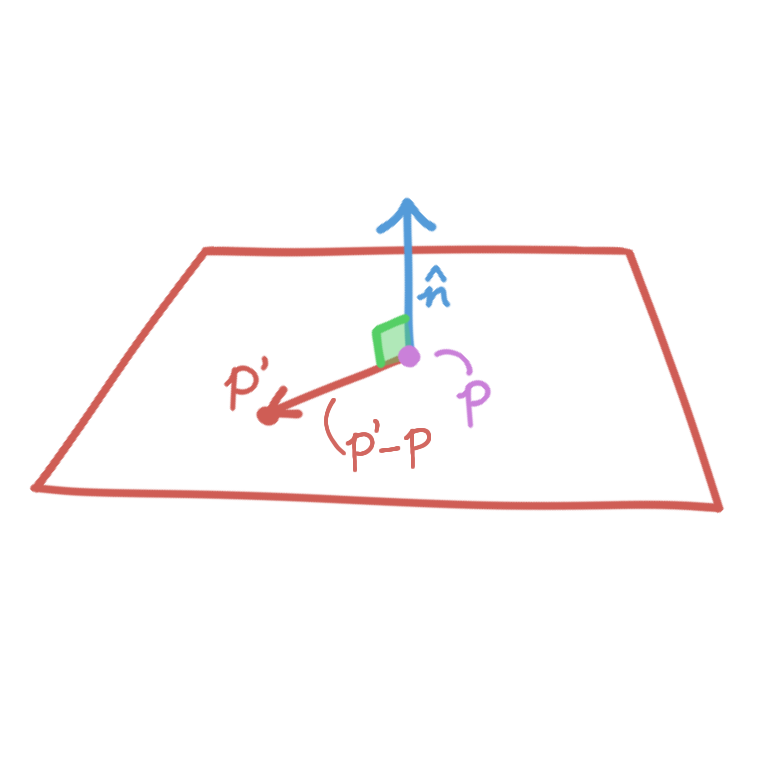
\includegraphics[width=13em, height=13em]{primitive_geometry_point_normal_plane}
\end{center}

\begin{center}
    $(P' - P) \cdot \hat{n} = 0$
\end{center}

where:
\begin{itemize}
    \item $P'$: is any point on the plane.
    \item $\hat{n}$: is the unit vector that represents the direction / facing of the plane.
    \item $P$: is an already known point on the plane.
\end{itemize}

Recall that dot product of two vectors gets the "parallelness" of two vectors,
if two vectors are perpendicular, their dot product should be 0, which makes sense for any point of a plane
if we draw a vector from point $P$ to point $P'$, the vector should lie on the plane.



\subsubsection{Ray-Plane Intersection for Distance-Normal Form}
We can replace the $P$ in plane's Distance-Norm formula with the Ray's formula with respect to points along the ray.

TODO: image here :3

\begin{center}
    $(O + \hat{D}t) \cdot \hat{n} - d = 0$
\end{center}

Since, $O,\hat{D}$ and $\hat{n}$ are known when calculating the intersection,
we solve for $t$:

\begin{center}
    $t = \frac{d - \hat{n} \cdot O}{\hat{n} \cdot \hat{D}}$
\end{center}

If $t \geq 0$ then the intersection is either at the beginning of the ray($t=0$) or
in front of the ray.
If $t < 0$ then the intersection is behind the ray's direction.

\sgap

If $\hat{n} \cdot \hat{D} = 0$ then we know that the ray is actually perpendicular with
the plane's surface direction. It either misses entirely, or hits infinite points.

\sgap

After figuring out a valid value for $t$, obtaining the point of intersection should be as simple as
plugging(substituting) the value $t$ in the original Ray formula:

\begin{center}
    $P_{intersect}=O+\hat{D}t_{found}$
\end{center}

$P_{intersect}$ should be the exact point of intersection on the plane!

\subsubsection{Converting between Point-Normal form and Distance-Normal form}
TODO: $d=O \cdot \hat{n}$ and $O = d \hat{n}$

\subsubsection{Ray-Plane Intersection for Point-Normal Form}
Much like the Distance-Normal form, we can also replace the $P$ in plane's Point-Norm formula with the Ray's formula with respect to points along the ray.

TODO: image here :3

\begin{center}
    $(O + \hat{D}t - P) \cdot \hat{n} = 0$
\end{center}

Solving for $t$ we get:
\begin{center}
    $t = \frac{(P - O) \cdot \hat{n}}{\hat{D} \cdot \hat{n}}$
\end{center}

The rest should be exactly the same as Distance-Normal form Ray-Plane intersection :3


\subsubsection{Mirroring a Point with regards to the Plane}
If you think about mirrors, they "imitate" everything from one side, just "mirrored" / "flipped" using the mirror itself
as a center for flipping. We can think of a plane as a mirror in 3D space, we can mirror any point from one side to the other side
of the "mirror"(plane) using some formula :O

\sgap
The formula for mirroring a point in \textbf{Point-Normal form} for the plane should be as follows:
\begin{center}
    $P' = P - 2 \hat{n} [(P - O) \cdot \hat{n}]$
\end{center}

where:
\begin{itemize}
    \item $P$: is the initial point to mirror.
    \item $P'$: is the final point that got mirrored.
    \item $\hat{n}$: is the normal / direction that the plane is facing.
    \item $O$: is any known point on the plane.
\end{itemize}

This is how it looks like visually:

TODO: put an image here showing the plane, the point $P$ and the reflected point $P'$, and also the projected vector
$\hat{n}[(P - O) \cdot \hat{n}]$





\subsubsection{Plane from two different, non-zero vectors}
You can also define a plane's facing direction with two different, non-zero vectors, in mathematical terms:

TODO: image here :3

\begin{center}
    $\hat{n} = \frac{\vec{a} \times \vec{b}}{\|\vec{a} \times \vec{b}\|}$
\end{center}

where $\vec{a} \neq \vec{b}, \|\vec{a}\| \neq 0, \|\vec{b}\| \neq 0$




\subsection{Sphere}
A sphere is defined as all the points $P$ at an equal distance $r$
from the center point $C$:

\begin{center}
    $\|P-C\|-r=0$
\end{center}

where:
\begin{itemize}
    \item $P$: is any point on the surface of the sphere.
    \item $C$: is the center of the sphere.
    \item $r$: is the radius of the circle, from the center $C$ to any point on the
        surface of the sphere $P$.
\end{itemize}

\subsubsection{Ray-Sphere Intersection}
TODO

\subsection{Axis-Aligned Bounding Box}
TODO

\subsection{Triangle}
TODO

\subsection{Barycentric Coordinates}
TODO



\section{Finite Rotations in 3D}
There's actually multiple ways to represent rotation in 3D space, this section explains
multiple ways of representing rotations, and specifically to rotate vectors, points and or objects in 3D eucledian space.

\subsection{Euler's Rotation Theorem}
This theorem states that given two orientations in 3D space $R_1$ and $R_2$,
then there exist an axis $\hat{A}$ and an angle $\theta$ such that it runs through a fixed point
and when applying the rotation around the axis $\hat{A}$ of $\theta$ amount to the orientation $R_1$ gives $R_2$.

In laymans' terms, you can always find a pair of axis-angle to get from one orientation to another with just 1 rotation.

\subsection{Euler-Rodrigues' Finite Rotation Formula}
Euler-Rodrigues' Finite Rotation Formula states that given a vector $\vec{v}$, we can
obtain the rotated vector $\vec{v'}$ by rotating it around an axis which is denoted by
a unit vector $\hat{k}$ of an angle of $\theta$.

\begin{center}
    $\vec{v'}=\vec{v}~cos~\theta + (\hat{k} \times \vec{v})~sin~\theta + \hat{k}(\hat{k} \cdot \vec{v})(1 - cos~\theta)$
\end{center}

where:
\begin{itemize}
    \item $\vec{v}$: is the vector to rotate.
    \item $\vec{v'}$: is the resulting rotated vector along the axis.
    \item $\hat{k}$: is the unit vector denoting the axis of rotation.
    \item $\theta$: is the angle of rotation to apply to the vector around the axis $\hat{k}$.
\end{itemize}

It is also useful to define $\hat{k}$ with respect to two non-zero vectors $\vec{a}$ and $\vec{b}$ ($\vec{a} \neq \vec{b}$) which
can denote a plane of rotation:

\begin{center}
    $\hat{k} = \frac{\vec{a} \times \vec{b}}{\|\vec{a} \times \vec{b}\|}$
\end{center}

\vspace{.5em}

\emph{
    NOTE: The formula shown above is more computationally efficient compared to
    other means of rotation.
}





\newpage
\input{geometric_algebra}

\newpage
\input{complex_numbers}

\newpage
\chapter{Quaternions}
Quaternions are four dimensional complex numbers that is defined as the following:

\begin{center}
    $Q = w + a\mathbf{i} + b\mathbf{j} + c\mathbf{k}=\begin{bmatrix}w & \begin{pmatrix}a & b & c\end{pmatrix}\end{bmatrix}=\begin{bmatrix}w & \vec{V}\end{bmatrix}$
\end{center}

where:
\begin{itemize}
    \item $w, a, b, c$: are the real numbers $\mathbb{R}$ that denotes the weight of each axis in the complex number.
    \item $\mathbf{i}, \mathbf{j}, \mathbf{k}$: are the axes representing the 2nd up to 4th dimensions. ($w$ is it's own dimension as well! In the real dimension :3)
    \item satisfies $\mathbf{i}^2=\mathbf{j}^2=\mathbf{k}^2=\mathbf{ijk}=-1$
    \item $\vec{V}$: is referred to as the \textbf{vector component} of a quaternion.
    \item $w$: is referred to as the \textbf{scalar component} of a quaternion.
\end{itemize}



\subsection{Quaternion Properties}

\textbf{Magnitude} of a quaternion:
\begin{center}
    $\|Q\| = \|\begin{bmatrix}w & \vec{V}\end{bmatrix}\| = \sqrt{w^2 + \|\vec{V}\|^2}$
\end{center}

If we define $\vec{V} = \begin{bmatrix}a & b & c\end{bmatrix}$ then:
\begin{center}
    $\|Q\| = \sqrt{w^2 + a^2 + b^2 + c^2}$
\end{center}

Which is similar to a four dimensional vector's eucledian / pythagorean distance.

If the magnitude of a quaternion is $1$, then we call it a \textbf{unit quaternion}(similar to a unit vector).

A unit quaternion is special, as it represents "pure rotation", or "rotational displacement" for
three-dimensional spaces.

\sgap
\textbf{Identity} quaternion:
\begin{center}
    $I = \begin{bmatrix}1 & \vec{0}\end{bmatrix}$
\end{center}

The identity quaternion is special because it means "\textbf{no rotational displacement}", it
is particularly important with quaternion inverses and multiplication (see \textbf{Quaternion Operations} section for more detail).


\subsection{Quaternion Operations}
\textbf{Scalar Multiplication} of a quaternion:
\begin{center}
    $kQ = k \begin{bmatrix}w & \vec{V}\end{bmatrix} =\begin{bmatrix}kw & k\vec{V}\end{bmatrix}$
\end{center}


\textbf{Scalar Division} of a quaternion:
\begin{center}
    $\frac{Q}{k} = \frac{\begin{bmatrix}w & \vec{V}\end{bmatrix}}{k} =\begin{bmatrix}\frac{w}{k} & \frac{1}{k}\vec{V}\end{bmatrix}$
\end{center}

\sgap
\textbf{Multiplication} between two quaternions:
\begin{center}
    \begin{flalign}
        Q_1Q_2 & = \begin{bmatrix}w_1 & \vec{V_1}\end{bmatrix}\begin{bmatrix}w_2 & \vec{V_2}\end{bmatrix} \\
            & = \begin{bmatrix}w_1w_2 - \vec{V_1} \cdot \vec{V_2} & w_1\vec{V_2} + w_2\vec{V_1} + \vec{V_1} \times \vec{V_2}\end{bmatrix}
    \end{flalign}
\end{center}

That's quite long isn't it? Notice that the vector part has $\vec{V_1} \times \vec{V_2}$, this means
quaternions actually are non-commutative(because vector cross products are non-commutative)! So in mathematical terms:

\begin{center}
    $Q_1Q_2 \neq Q_2Q_1$
\end{center}

But do not worry! Quaternion multiplication is actually associative:
\begin{center}
    $(Q_1Q_2)Q_3 = Q_1(Q_2Q_3)$
\end{center}

Just be careful when rearranging or calculating quaternion equations :D


\sgap
\textbf{Conjugate} of a quaternion:
\begin{center}
    $Q^* = \begin{bmatrix}w & \vec{V}\end{bmatrix}^* =\begin{bmatrix}w & -\vec{V}\end{bmatrix}$
\end{center}

The conjugate of a quaternion simply negates the vector component of a quaternion.

\sgap
\textbf{Inverse} of a quaternion:
\begin{center}
    $Q^{-1} = \frac{Q^*}{\|Q\|^2}$
\end{center}

The inverse of a quaternion applies the "inverse" rotation of a regular quaternion,
if a quaternion $Q$ is inversely applied to itself, then we would get the \textbf{identity} quaternion:
\begin{center}
    $QQ^{-1} = Q^{-1}Q = I = \begin{bmatrix}1 & \vec{0}\end{bmatrix}$
\end{center}

For a unit quaternion, due to the fact that it's magnitude being 1, it's inverse
is simply the conjugate of the quaternion!

\sgap
\textbf{Dot Product} of a quaternion:
\begin{center}
    $Q_1 \cdot Q_2 = \begin{bmatrix}w_1 & \vec{V_1}\end{bmatrix} \cdot \begin{bmatrix}w_2 & \vec{V_2}\end{bmatrix} = w_1w_2 + \vec{V_1} \cdot \vec{V_2}$
\end{center}

The quaternion dot product, similar to a vector dot product, also does element-wise multiplication, and returns a scalar
and not a quaternion.


\subsection{Quaternions as Rotations for 3D spaces(Versors)}
When we use unit quaternions for the purpose of rotating vectors, points or objects in three-dimensional spaces
, this unit quaternion is also called a "\textbf{versor}".

A versor can be defined using \textbf{Angle-Axis Form}:
\begin{center}
    $q = \begin{bmatrix}w & \vec{V}\end{bmatrix}=\begin{bmatrix}cos~\frac{\theta}{2} & sin~\frac{\theta}{2}~\hat{n}\end{bmatrix}$
\end{center}

where:
\begin{itemize}
    \item $q$: is the versor itself(or the unit quaternion).
    \item $\hat{n}$: the axis of rotation denoted as a unit vector.
    \item $\theta$: the angle of rotation around the axis denoted by $\hat{n}$.
\end{itemize}

The versor represents a pure \textbf{rotational displacement}, which can be visualized like this:
\begin{center}
    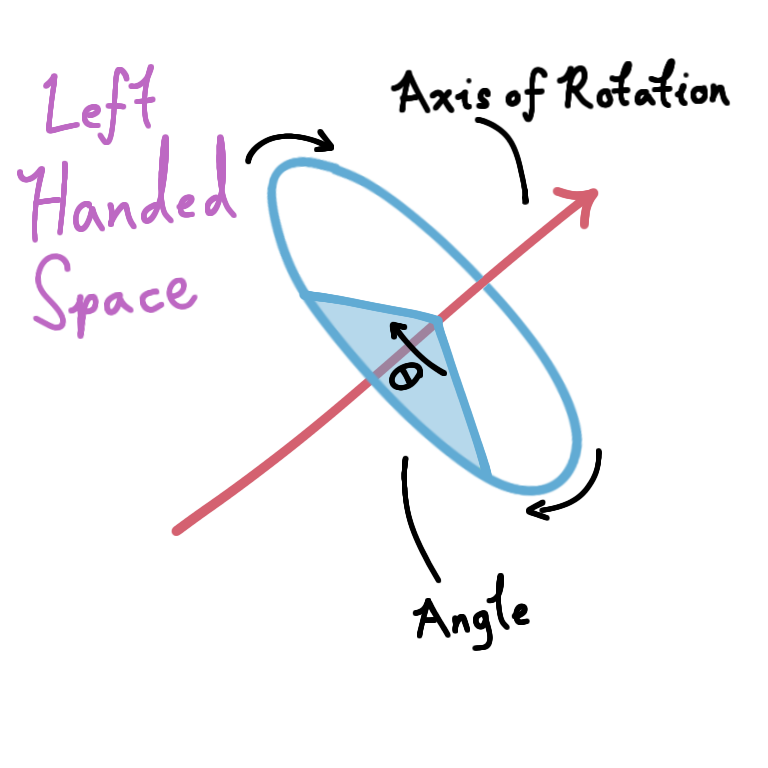
\includegraphics[width=13em, height=13em]{axis_angle_rotation}
\end{center}


You can quickly observe that:
\begin{center}
    $w = cos~\frac{\theta}{2},~ \vec{V} = sin~\frac{\theta}{2} \hat{n}$
\end{center}

You can apply a rotation to a 3D point $P=\begin{pmatrix}x & y & z\end{pmatrix}$ by first promoting this
point into a quaternion with the real component($w$) set to zero:
\begin{center}
    $P_q = \begin{bmatrix}0 & \begin{pmatrix}x & y & z\end{pmatrix}\end{bmatrix}$
\end{center}

Then apply this new promoted point quaternion in this "weird-looking" formula given a versor $Q$:
\begin{center}
    $P_q' = QP_qQ^{-1} = \begin{bmatrix}w' & \begin{pmatrix}x' & y' & z'\end{pmatrix}\end{bmatrix}$
\end{center}

The result new quaternion $P_q'$ should have the result rotated point $P'$ in it's vector component of $P_q'$.
In mathematical terms:
\begin{center}
    $P' = \begin{pmatrix}x' & y' & z'\end{pmatrix}$
\end{center}

\sgap

This formula can actually be applied multiple times consecutively to create a new rotational displacement
that is the "sum" of all of each individual rotation:
\begin{center}
    \begin{flalign}
        P_q & = b(aPa^{-1})b^{-1} \\
            & = (ba)P(a^{-1}b^{-1}) \\
            & = (ba)P(ba)^{-1}
    \end{flalign}
\end{center}

The above equation applies the versor $a$ first on $P$, then applies versor $b$ afterwards.
By rearranging the equation, it is obvious that it is equivalent to rotating the combination of two
versors $a$ and $b$.

\sgap
\subsection{Logarithm and Exponential Functions of Quaternions}

If we let $\alpha = \frac{\theta}{2}$, then we can define the logarithm function of a versor $Q$ as:
\begin{center}
    $log(Q) \equiv log(\begin{bmatrix}cos~\alpha & sin~\alpha~\hat{n}\end{bmatrix}) = \begin{bmatrix}0 & \alpha\hat{n}\end{bmatrix}$
\end{center}

As you can see, the logarithm of a versor is simply storing the half angle of rotation directly in the unit vector!
And because we know unit vectors always have a length of 1, we can obtain back the half angle $\alpha$
by simply getting the magnitude of the vector part of the quaternion(note that the magnitude
of a vector is always positive, therefore we will always lose the sign of the angle!)

But do not worry, the sign is preserved on the unit vector instead! You can see it as rotating on the opposite direction
with the reverse angle(i.e. $-\alpha$ with $-\hat{n}$).

It is also important to note the result may not be a versor / unit quaternion!

This method of storing more information in less numbers is commonly referred to as \textbf{exponential map format}.

\tgap
If a quaternion has the format $Q = \begin{bmatrix}0 & \alpha\hat{n}\end{bmatrix}$
then we can define the exponential function of a quaternion as:

\begin{center}
    $exp(Q) \equiv exp(\begin{bmatrix}0 & \alpha\hat{n}\end{bmatrix}) = \begin{bmatrix}cos~\alpha & sin~\alpha~\hat{n}\end{bmatrix}$
\end{center}

Hopefully you have noticed by now that the logarithm and exponential functions are actually inverse of each other:

\begin{center}
    $exp(log(Q)) = Q$
\end{center}

\sgap
\subsection{Exponentiation of Quaternions}
Confusingly, quaternions also have exponentiation, it is different compared to the \textbf{exponential} function. It is mathematically defined as:
\begin{center}
    $Q^t \equiv exp(t~log(Q))$
\end{center}

When applying exponentiation of $t$ to a versor that rotates $\theta$ angle around an axis, the resulting quaternion rotates
$\theta t$... With a catch! If $\theta > 180~degrees$ then what happens, is the quaternion kind of "flips to the other direction",
and rotates in the "shorter angle", here's an image that shows this:

TODO: put image here :)

So if $Q$ rotates 50 degrees, then $Q^2$ rotates 100 degrees, but $Q^4$ does not rotate 200 degrees, but rather $200 - 360 = -160~degrees$
on the other direction! (because it is shorter)

\subsection{Quaternion Difference}
TODO: Explain $\delta d = ba^{-1}$

\subsection{Quaternion Interpolation(Spherical Interpolation)}
TODO: use the above explanation of difference to derive interpolation


\newpage
\chapter{Shading Models}

\section{Phong Shading Model}
TODO

\section{Blinn-Phong Shading Model}
TODO


\newpage
\chapter{Useful Resources and References}

\begin{enumerate}
    \item Book: \emph{3D Math Primer for Graphics and Game Development} by Fletcher Dunn and Ian Parberry
\end{enumerate}


\end{document}
